\section{Expérimentations et Usages}
\subsection{Lancement de l'application}
Vous devez ouvrir un terminal à l'emplacement du dossier.

Pour :
\begin{itemize}
\item Lancer l'application sur le terminal : exécuter \verb|ant runConsol|
\item Lancer l'application avec l'interface graphique: exécuter \verb|ant runInterface|
\item Initialiser le projet : exécuter \verb|ant init| . Cette initialisation créera les dossiers de base bin, doc et dist.
\item Compiler le projet : exécuter \verb|ant compile| 
\item Générer la Javadoc : exécuter \verb|ant javadoc|
\item Générer le fichier jar : exécuter \verb|ant packaging|
\item Nettoyer le projet : exécuter \verb|ant clean|
\item Lancer les tests : exécuter \verb|ant test|
\end{itemize}
\subsection{Implémentation de l'Interface graphique}
Java Swing est l'interface que nous avons choisie pour faire l'implémentation graphique de notre simulateur. Nous y avons défini 5 classes dans le package \texttt{views} et une classe \texttt{Aide} dans le package \texttt{util}.

\texttt{Views} contient les classes suivantes :

\begin{enumerate}
\item \texttt{Config} : permet de configurer le jeu en définissant les règles et le type de voisinage utilisé, et de voir l'évolution de la simulation (cellule vivante, nombre de générations, ainsi que la vitesse de l'algorithme choisi). Elle contient également un bouton qui permet d'initialiser la grille avec une configuration aléatoire.
\item \texttt{GridGraphique} : représente la grille graphique. Elle dispose d'une fonction qui permet de cliquer sur la grille pour changer l'état de la cellule.
\item \texttt{Rendu} : cette classe est divisée en 3 parties : une pour contenir les boutons de navigation, une pour la grille, et une dernière permettant à l'utilisateur de choisir l'algorithme utilisé pour la simulation.
\item \texttt{Menu} : cette classe permet à l'utilisateur de choisir dans une liste de motifs prédéfinis et un bouton d'aide qui explique l'utilisation correcte de l'application.
\item \texttt{MainWindow} : est la classe principale qui compose l'ensemble des composants de l'interface graphique. Elle met en liaison la partie interface graphique et le modèle du simulateur (\texttt{game}).
\end{enumerate}

\texttt{Util} contient la classe suivante :

\begin{itemize}
\item \texttt{Aide} : cette classe importe un fichier texte expliquant le bon fonctionnement du simulateur.
\end{itemize}
\subsection{Fonctionnement de l'interface graphique}
Au lancement du programme, une fenêtre s'affiche, comme illustré dans la figure ci-dessous. Cette fenêtre permet aux utilisateurs de commencer une nouvelle partie. Les utilisateurs ont le choix entre deux boutons pour choisir entre le jeu classique et le jeu avec Hashlife.

\begin{figure}[h]
\centering
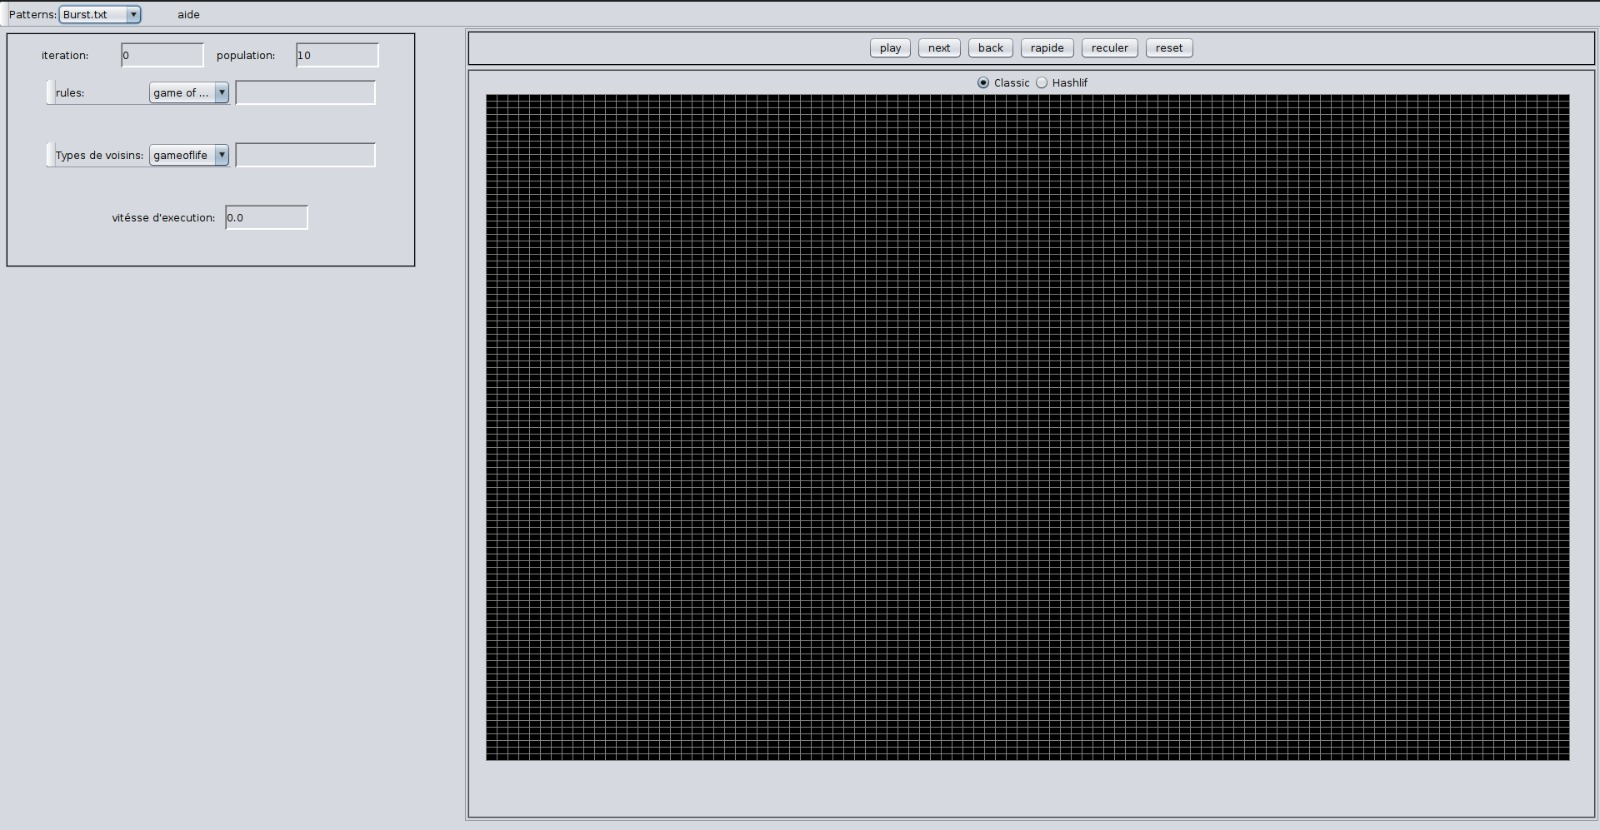
\includegraphics[width=11cm]{images/image0.JPG}
\caption{Lancement du jeu}
\end{figure}

La fenêtre comprend également les éléments suivants :

\begin{itemize}
\item Les boutons de contrôle, qui permettent de démarrer/arrêter(play/stop) la simulation, avancer/reculer(next/back) d'une génération, accélérer/ralentir(rapide/reculer) la simulation et restaurer(reset) la grille. Le bouton "Aide" redirige vers une fenêtre d'aide pour une utilisation optimale de l'application
\item La liste de patterns disponibles(patterns), qui permet aux utilisateurs de choisir un modèle prédéfini.
\item Les boutons de règles(rules), qui permettent aux utilisateurs de choisir la règle utilisée pour la simulation (Game of Life par défaut).
\item Les boutons de type de voisins, qui permettent aux utilisateurs de choisir le type de voisinage utilisé (game of life par défaut).
\item Le contrôle de la vitesse d'exécution, qui permet aux utilisateurs de visualiser la vitesse à laquelle la simulation avance selon l'algorithme utilisé.
\item initialisation de la grille : pour initialiser la grille il est possible de  cliquer sur le bouton "Init random" pour initialiser la grille avec des cellules aléatoires, ou sélectionner un pattern existant dans la liste,
ou encore cliquer directement sur les cellules de la grille pour les activer/désactiver
\end{itemize}
\newpage
\begin{figure}[h]
\centering
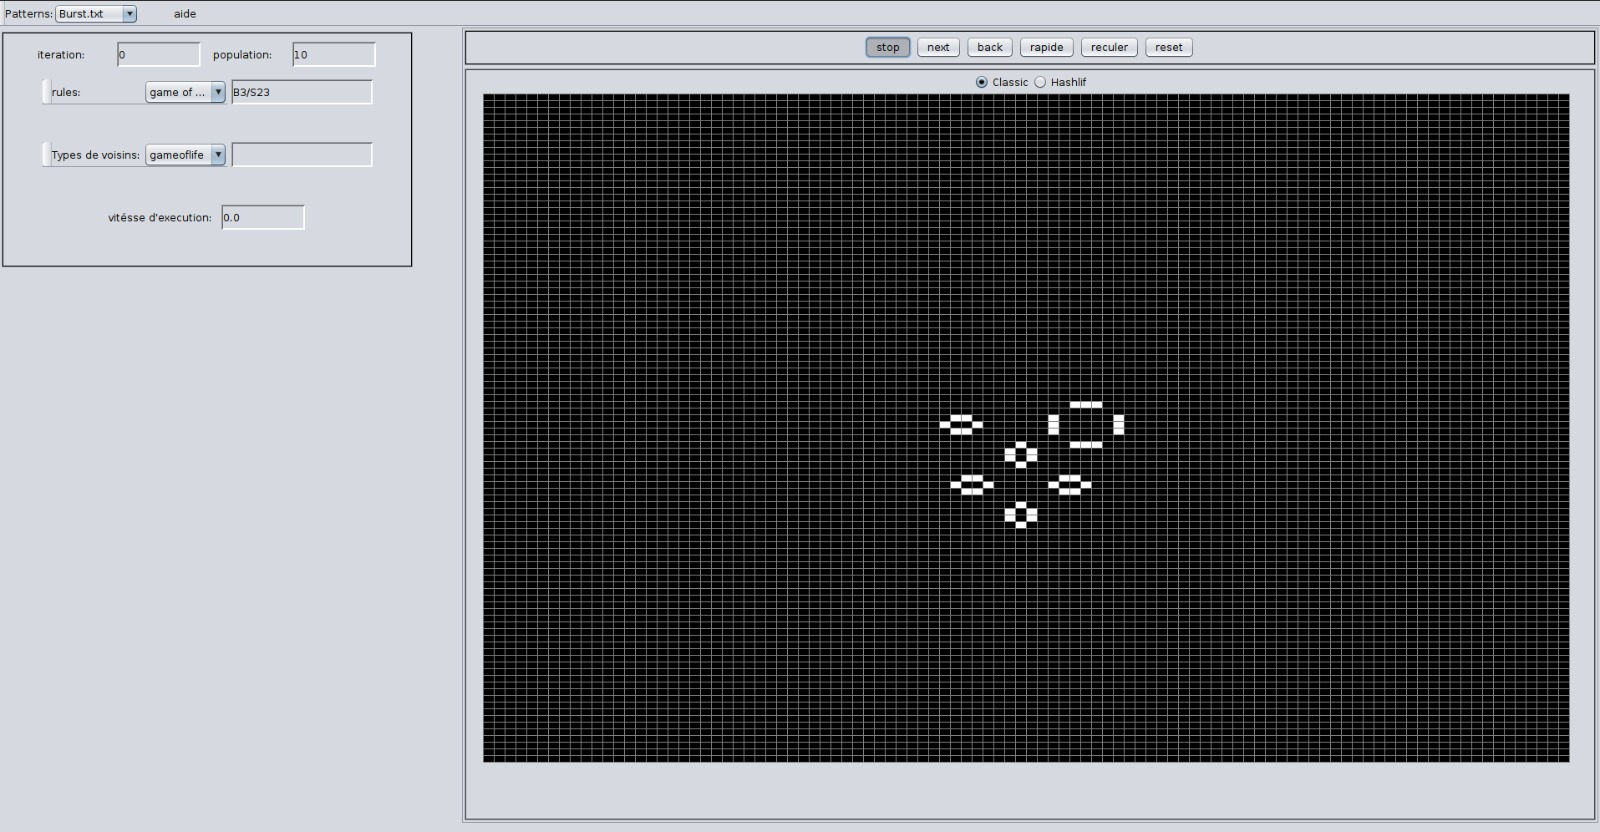
\includegraphics[width=11cm]{images/image2.jpeg}
\caption{Illustration du bouton "play"}
\end{figure}

\begin{figure}[h]
\centering
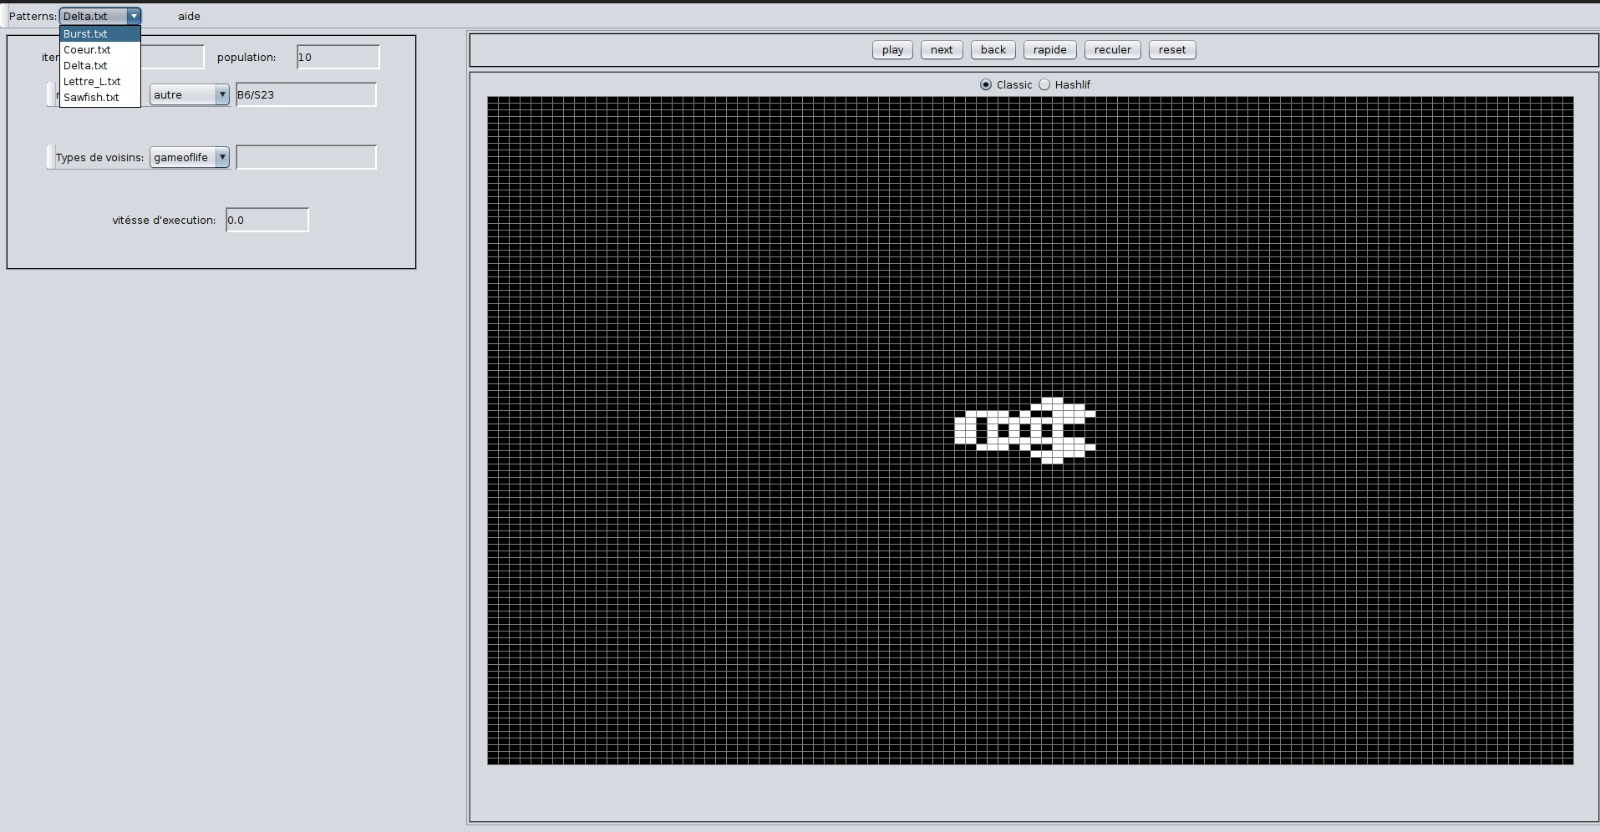
\includegraphics[width=11cm]{images/image4.jpeg}
\caption{Illustration de la liste de patterns disponibles}
\end{figure}
\newpage
\begin{figure}[h]
\centering
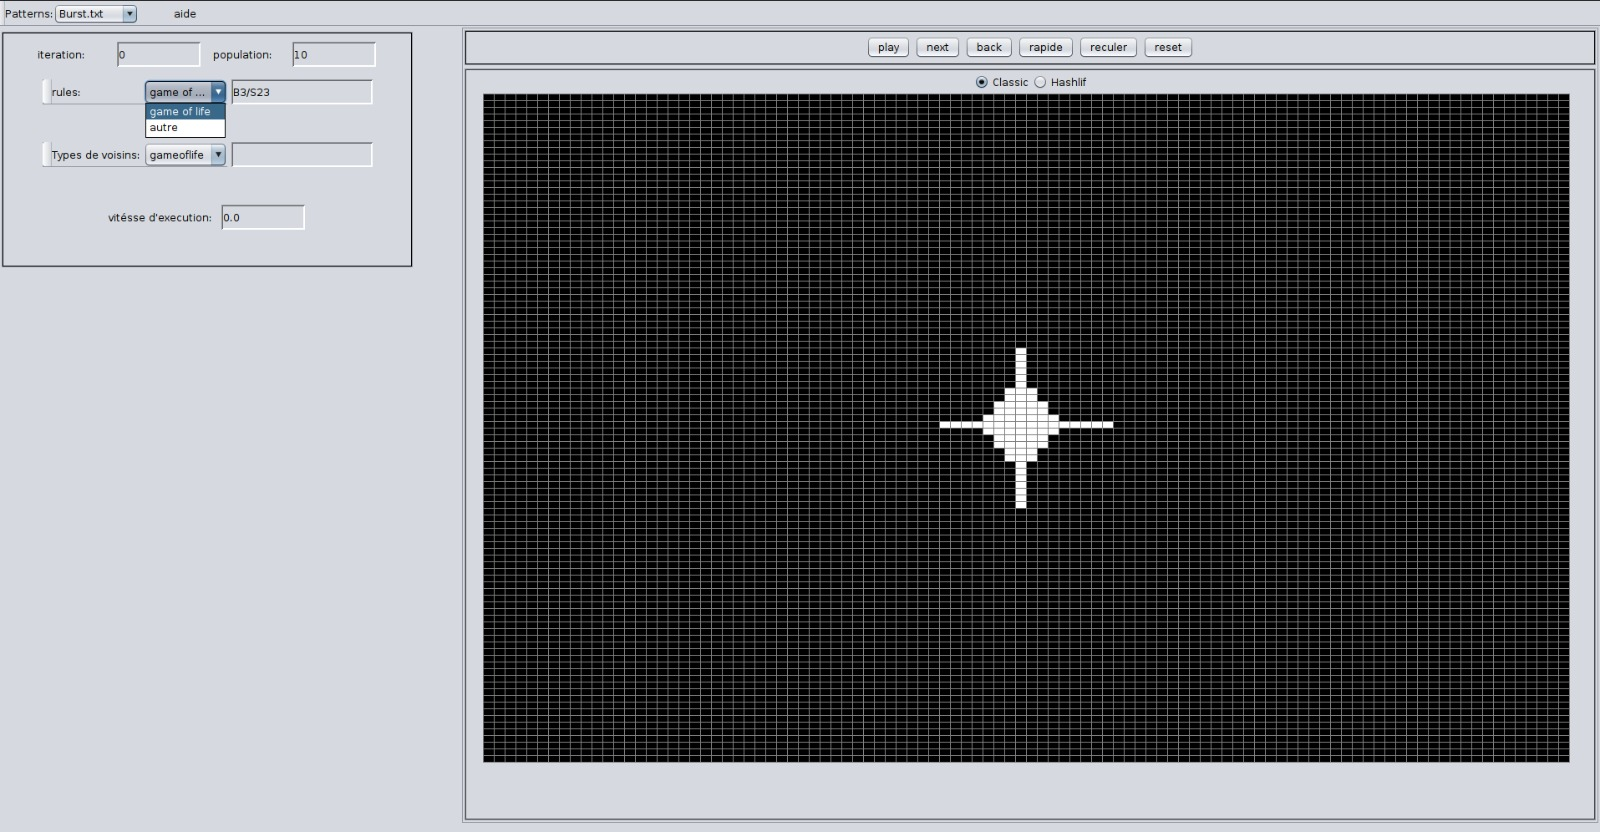
\includegraphics[width=11cm]{images/image3.jpeg}
\caption{Illustration du bouton "rules"}
\end{figure}
\begin{figure}[h]
\centering
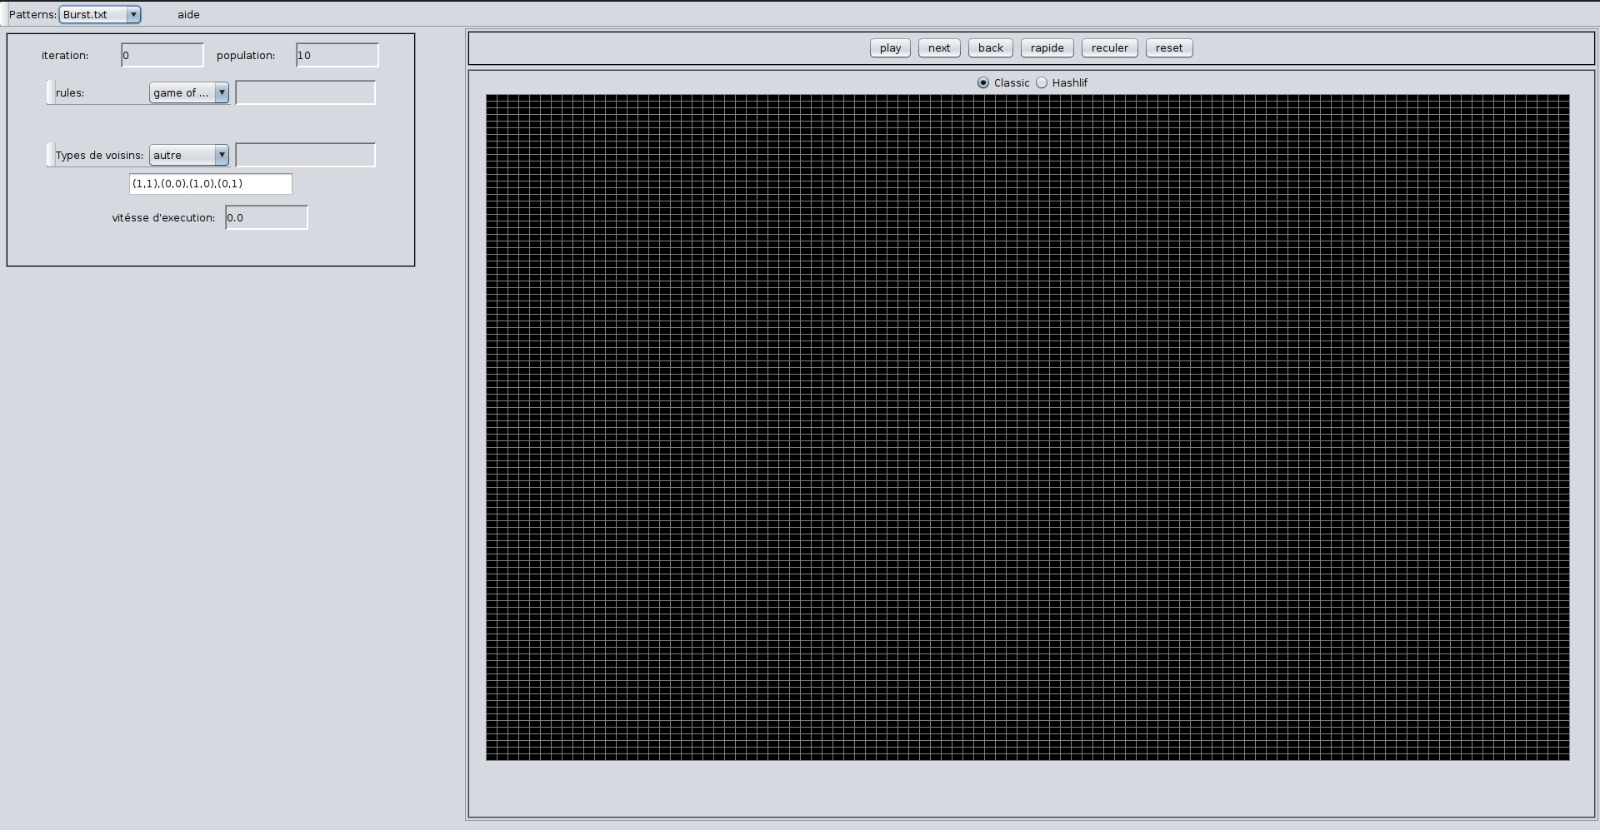
\includegraphics[width=11cm]{images/image5.JPG}
\caption{Illustration du bouton "type de voisins"}
\end{figure}
\subsection{Test du Logiciel}
Nous avons utilisé le framework open source JUnit 4.12 pour réaliser nos tests unitaires. Ces tests portent sur l'ensemble des méthodes essentielles pour le bon fonctionnement de notre projet
\newpage
\begin{figure}[h]
\centering
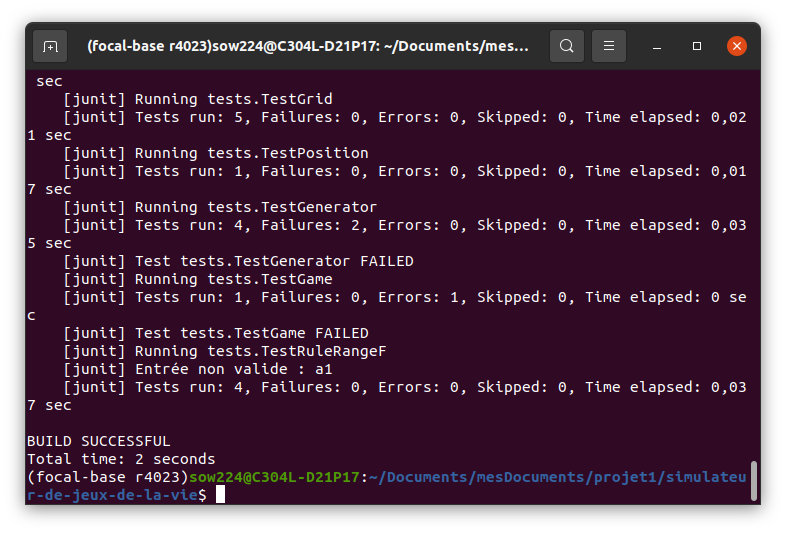
\includegraphics[width=11cm]{images/Capture d’écran de 2023-04-20 21-15-04.png}
\caption{test"}
\end{figure}